%% Template for EU deliverable, using the deliverable.sty style file

\documentclass[12pt,a4paper,twoside]{article}

%% common package
\usepackage[headers]{deliverable}
\usepackage{xspace}
\usepackage{verbatim}
\usepackage[usenames]{color}
\usepackage[usenames,dvipsnames]{xcolor}
\usepackage{graphicx}
\usepackage{url}
\usepackage{array}
\usepackage{amsmath,bm,amsfonts}
\usepackage{tikz}
\usetikzlibrary{arrows,automata}
%%

%%insert here other packages needed by sections

%%

%%%%%%%%%%%%%%%%%%%%%%%%%%%%%%%%%%%%%%%%%%%%%%%%%%%%%%%%%%%%%%%%%%%%%%%%%%%%%%
%%% Titlepage
%%%%%%%%%%%%%%%%%%%%%%%%%%%%%%%%%%%%%%%%%%%%%%%%%%%%%%%%%%%%%%%%%%%%%%%%%%%%%%

% declaration of variables used in style
\deliverableDocnumber{D5.1}
\deliverableTitle{Validation scenario 1: balancing on multiple rigid contacts}

\deliverableAuthor{Francesco Nori}
\deliverableResponsiblePartner{IIT}
\deliverableAffiliation{% Insert here authors affiliations
 $^1$ IIT
}

\deliverableReviewer{Francesco Nori}
\deliverableCoordinator{Francesco Nori}
\deliverableActivityNumber{n} %% n=1,..,10
\deliverableActivity{RTD}
\deliverableDoctype{Deliverable} %% or Prototype
\deliverableClassification{Public} % or Consortium
\deliverableDistribution{Consortium} %
\deliverableStatus{Draft} % Draft or Final
\deliverableDeliveryDate{28/2/2014}
\deliverableFile{D5.1.pdf} % please do not use "-" in the name
\deliverableVersion{1.0}
\deliverableDate{Feb.~28, 2014}
\deliverableYear{2014}
\deliverablePages{\pageref{LastPage}}
\deliverableChangelog{v.1.0 & Feb 19, 2014 & First draft %%\\\hline
%%              v.2.0 & Feb 20, 2007 & Final version
}
\deliverableProjectStartingDate{1st March 2013}
\deliverableProjectEndDate{28th February 2017}
\deliverableProjectAcronym{CoDyCo}
\deliverableProjectTitle{Whole-Body Compliant Dynamical Contacts in Cognitive Humanoids}
 \deliverableContractNumber{600716}
 \deliverableProjectCoordinator{Istituto Italiano di Tecnologia}
 \deliverableProjectUrl{www.codyco.eu}
 \deliverableFrameworkProgramme{FP7}
 
 \deliverableWorkpackage{deliv WP5}
 \deliverableEditors{Francesco Nori}
 \deliverableContributors{Francesco Nori, Andrea Del Prete, Daniele Pucci, Serena Ivaldi, Vincent Padois}
 \deliverableReviewers{}
\deliverableAbstract{In the present deliverable we discuss the technical details and choices for the implementation of on the year-1 validation scenario of the CoDyCo project. This validation scenario consists on balancing with multiple rigid contact points. Contact and trajectory planning is not part of the scenario. The final validation consists in controlling the iCub across the following sequence of control tasks. Multiple (force and position) tasks will be handled with strict priorities by adopting the theoretical framework known as stack of tasks \cite{delPrete2013}. First the robot is standing on two feet and, in order to maintain this posture, a controller takes care of controlling the left and right foot position and forces exchanged with the ground. Second, the robot start moving both hands towards a table with the intend of establishing two additional support contacts: in this phase the robot starts controlling also the hands Cartesian position. As soon as the artificial skin detects the contact between the hands and the table the controllers starts including hands force regulation among the control tasks.}
\deliverableReviewers{}
\deliverableKeywordList{Multiple, rigid, contacts, control, stability, tracking, forces, torques.}

%%%%%%%%%%%%%%%%%%%%%%%%%%%%%%%%%%%%%%%%%%%%%%%%%%%%%%%%%%%%%%%%%%%%%%%%%%%%%%
%%% Sections
%%%%%%%%%%%%%%%%%%%%%%%%%%%%%%%%%%%%%%%%%%%%%%%%%%%%%%%%%%%%%%%%%%%%%%%%%%%%%%

%% constants
\newcommand{\botegoCaps}{BOTEGO}
\newcommand{\certhCaps}{CERTH}
\newcommand{\cybionCaps}{CYBION}
\newcommand{\nuigCaps}{NUIG}
\newcommand{\ubitechCaps}{UBITECH}

%%
%%%%%%%%%%%%%%%%%%%%%%%%%%%%%% BEGIN DOCUMENT
\begin{document}

\deliverableMaketitle

%%TODO move to style
\newcolumntype{L}[1]{>{\raggedright\let\newline\\\arraybackslash\hspace{0pt}}m{#1}}
\newcolumntype{C}[1]{>{\centering\let\newline\\\arraybackslash\hspace{0pt}}m{#1}}
\newcolumntype{R}[1]{>{\raggedleft\let\newline\\\arraybackslash\hspace{0pt}}m{#1}}

\textbf{Document Revision History}
\begin{center}
\begin{tabular}{|C{2cm}|C{3cm}|p{5cm}|C{4cm}|}
\hline
\textbf{Version}&\textbf{Date}&\textbf{Description}&\textbf{Author}\\\hline
First draft & 19 Feb 2014 & In this version we simply write down a few considerations on the first year validation scenario as discussed after the mid-year CoDyCo meeting in Paris. & Francesco Nori \\\hline
\end{tabular}
\end{center}
 
 \clearpage

\newpage
\renewcommand*\contentsname{Table of Contents}
\renewcommand*\listfigurename{Index of Figures}
\tableofcontents
\newpage
\newpage

%%%%%%%%%%%%%%%%%%%%%%%% Start deliverable content here.

\section{Introduction}

The first year CoDyCo validation scenario deals with iCub balancing on multiple rigid contacts. The theoretical framework for dealing with these kind of situations has been extensively explored in a number of papers \cite{Aghili2005,Righetti2013}. Taking advantage of our experience on the topic \cite{delPrete2013} the first year validation scenario will be implemented in the Task Space Inverse Dynamics (TSID) framework and in particular we will consider its application to floating base kinematic chains. The iCub will be torque controlled and the controller will assume that desired torques are exactly executed by a lower level torque control. Dynamics will be computed with a custom library, iDynTree\footnote{\url{http://wiki.icub.org/codyco/dox/html/group__iDynTree.html}}, built on top of KDL\footnote{\url{http://www.orocos.org/kdl}}. Desired joint torques will be computed by the TSID algorithm given a set of tasks and their relative priorities. The definition of tasks and priorities is described in details in the following sections. 

\section{Executive Summary}

The deliverable is organized as follows. Section \ref{sec:firstYearScenario} gives an high level presentation of the validation scenario to be presented at the first year review meeting. Section \ref{sec:TSID} discusses the numerical technique (TSID) used to implement the validation scenario as a prioritization of concurrent tasks. Section \ref{sec:tasks} discusses the set of control tasks that will be implemented in order to perform the validation scenario.  Their sequencing in the form of a finite state machine is discussed in Section \ref{sec:taskSequencing} and issues related to task switching discussed in Section \ref{sec:taskReferences}. Priorities between tasks are summarized in Section \ref{sec:taskPrioritization}.

\section{First Year Scenario Validation} \label{sec:firstYearScenario}

The first year scenario aims at validating on the iCub\footnote{ Implementation is foreseen on the iCub platforms currently available at IIT and UPMC.} the theoretical results of the consortium in performing the task of balancing on multiple rigid contacts. As clearly stated in the CoDyCo proposal the validation should not involve any planning and therefore the sequence of movements and trajectories will be predefined and kept constant across trials. During the mid-year meeting held in Paris, the sequence of movements was discussed and an agreement was found across the entire consortium. The scenario will begin with the iCub standing on two feet in front of an object that offers the possibility of additional contacts (e.g. a table where to place both hands). After some time the robot will start a movement of both hands towards the additional contact. As soon as the hands detect the additional contacts with the artificial skin, the iCub will start regulating the interaction forces at both hands trying to maintain a comfortable and stable posture.

\section{First year scenario implementation}

Recently we proposed a numerical technique \cite{delPrete2013} for solving the problem of controlling multiple concurrent tasks on floating base robots. Considered tasks include the control of contact forces and multiple motion tasks. Tasks are ordered according to a priority structure, with force tasks at the highest priority. The proposed solution, named task space inverse dynamics (TSID), is presented in the following section.

\subsection{Task Space Inverse Dynamics (TSID)} \label{sec:TSID}

Let's first recall how the force control problem is solved in the TSID framework in the context of floating base manipulators \cite{delPrete2013}. The framework computes the joint torques to match as close as possible a desired vector of forces at the contacts \eqref{eq:torquesTSID} compatible with the system dynamics \eqref{eq:dynTSID} and with the contact constraints \eqref{eq:contactTSID}:
\begin{subequations} \label{eq:TSID}
\begin{align} 
\label{eq:torquesTSID}
\bm {\tau}^* = \mbox{arg } \min_{\bm \tau \in \mathbb{R}^n}\,& \| \bm f - \bm f^*\|^2 \\
\label{eq:dynTSID}
s.t. \quad M \ddot{\bm q} + h - J_c^T \bm f & = S^T \bm \tau \\
\label{eq:contactTSID}
 J_c \ddot{\bm q} + \dot{J}_c \dot{\bm q} & = 0 \\
\label{eq:motionTSID}
 J_i \ddot{\bm q} + \dot{J}_i \dot{\bm q} & = \ddot {\bm x}_i^*, \qquad i = 1, \dots, N -1
\end{align}
\end{subequations}
where $\bm q$ is a vector of generalized coordinates describing the robot pose (includes both $\bm q_j$ and the floating base position), $\bm \tau$ is the vector of joint torques, $M$ is the mass matrix, $h$ contains both gravitational and Coriolis terms, $S$ is the selection matrix which takes into account the fact that we do not have a direct control over the floating base variables, $\bm f$ is the contact spatial vector, $\bm f^*$ is its desired value and $J_c$ is the contact Jacobian. 

In the TSID formalism, the idea is to solve the force control task (represented as in \eqref{eq:torquesTSID}) at the highest priority and to exploit the nullspace of this primary control task to perform $N-1$ motion tasks at lower priorities (represented as in \eqref{eq:motionTSID}). These tasks (indexed with $i = 1$, $\dots$, $N-1$) are all represented as the problem of tracking a given reference acceleration $\ddot {\bm x}_i^*$ for a variable ${\bm x}_i$ differentially linked to $\bm q$ by the Jacobian $J_i$, i.e. $\dot {\bm x}_i = J_i \dot {\bm q}$ and $\ddot {\bm x}_i = J_i \ddot {\bm q} + \dot J_i \dot {\bm q} $. Assuming that the force task has maximum priority the solution is the represented by the following expression:
\begin{equation}
\bm \tau^{*} = -(J_c\bar{S})^\top \bm f^* + N_j^{-1} {\ddot{\bm q}}_1^* + \bar{S}^\top h,
\end{equation}
where $\bar S = M^{-1} S^\top \left( S M^{-1} S^\top \right)^{-1}$ and the term ${\ddot{\bm q}}_1^*$ is computed solving the following recursion for $i =N$, $\dots$, $1$:
\begin{equation} 
\begin{split}
\ddot{\bm  q}_i =& \ddot{\bm q}_{i+1} + (J_i \bar{S} N_{p(i)})^\dagger+ (\ddot{\bm x}_i^*-\dot{J}_i\dot{\bm q} + J_i (U^T M_b^{-1}(h_b-J_{cb}^T f) - \bar{S} \ddot{\bm q}_{i+1}))\\
N_{p(i)} =& N_{p(i+1)} - (J_{i+1} \bar{S} N_{p(i+1)})^\dagger J_{i+1} \bar{S} N_{p(i+1)}, \\
%N_{p(i)} =& I - \sum_{j=i+1}^{N}(J_j \bar{S} N_{p(j)})^+ J_j \bar{S} N_{p(j)},
\end{split}
\end{equation}
which is initialized setting $\ddot{q}_{N+1} = 0$, \mbox{$N_{p(N)}=I$}, $J_N = J_c$ and $\ddot{ \bm x}_N = 0$.

\subsection{Set of admissible tasks} \label{sec:tasks}

The CoDyCo first year scenario is implemented within the TSID framework which requires the definition of a suitable set of position ($\ddot {\bm x}_i^*$) and force ($\bm f^*$) tasks and their relative priority. The set of admissible tasks is quite flexible also considering the flexibility of the underlying software libraries\footnote{\url{http://wiki.icub.org/codyco/dox/html/group__iDynTree.html}}. Nevertheless we list here a set of possible tasks, which we will use as a reference in the following sections. Quantities are defined as with a notation similar to the one used in \cite{featherstone2008}: $\bm v$  indicates a spatial velocity (a single vector for representing linear and angular velocities), $\bm a$  indicates a spatial acceleration (a single vector for representing linear and angular accelerations), $\bm f$ indicates a spatial force (a single vector for forces and torques), the index $i  =0$, $1$, $\dots$, $N_B-1$ is used to reference the $N_B$ rigid bodies representing the iCub body chain ($0$ being defined as the pelvis rigid link), the index $w$ is used to represent the world reference frame, the superscripts and subscripts $^{lh}$, $^{rh}$, $^{lf}$, $^{rf}$ indicate reference frames rigidly attached to the left hand, right hand, left foot and right foot respectively, the superscript $^{i}$ indicates the reference frame attached to the $i$-th rigid body, $^k {\bm X}_i$ represents the rigid roto-translation from the reference frame $i$ to the reference frame $k$, $\bm q_j$ represent the position of the iCub joints.

Tasks will be thrown out  of the following set of admissible tasks. For each task $T_i$ we specify the reference values ($\ddot {\bm x}_i$ or $\bm f^*$) and associated Jacobians ($J_i$). 
\begin{itemize}

\item $T^{rh}_{\bm X}$ : right hand linear and angular accelerations. 
\begin{eqnarray*}
\ddot {\bm x}^*_{i} &:& \qquad ^{rh}{\ddot {\bm x}}_w = ^{rh}{\ddot {\bm x}}^*_w, \quad {}^{rh}{\dot {\bm \omega}}_w = {}^{rh}{\dot {\bm \omega}}_w^*;\\
J_i &:& \qquad J_{rh};
\end{eqnarray*}

\item $T^{lh}_{\bm X}$ : right hand linear and angular accelerations. 
\begin{eqnarray*}
\ddot {\bm x}^*_{i} &:& \qquad ^{lh}{\ddot {\bm x}}_w = ^{lh}{\ddot {\bm x}}^*_w, \qquad {}^{lh}{\dot {\bm \omega}}_w = {}^{lh}{\dot {\bm \omega}}_w^* ;\\
J_i &:& \qquad J_{lh};
\end{eqnarray*}

\item $T^{com}_{\bm X}$ : center of mass acceleration. Move the center of mass with the following acceleration: 
\begin{eqnarray*}
\ddot {\bm x}^*_{i} &:& \qquad \ddot {\bm x}_{com} = \ddot {\bm x}_{com}^* ;\\
J_i &:& \qquad J_{com};
\end{eqnarray*}

\item $T^{rf}_{\bm f}$ : right foot force. Regulate the right foot interaction force to a predefined value: \begin{eqnarray*}
\ddot {\bm f}^*_{i} &:& \qquad {\bm f}_{rf} = {\bm f}^*_{rf} ;\\
J_i &:& \qquad J_{rf};
\end{eqnarray*}

\item $T^{lf}_{\bm f}$ : left foot force. Regulate the left foot interaction force to a predefined value: 
\begin{eqnarray*}
\ddot {\bm f}^*_{i} &:& \qquad {\bm f}_{lf} = {\bm f}^*_{lf} ;\\
J_i &:& \qquad J_{lf};
\end{eqnarray*}

\item $T^{rh}_{\bm f}$ : right hand force. Regulate the right hand interaction force to a predefined value: \begin{eqnarray*}
\ddot {\bm f}^*_{i} &:& \qquad {\bm f}_{rh} = {\bm f}^*_{rh} ;\\
J_i &:& \qquad J_{rh};
\end{eqnarray*}

\item $T^{lh}_{\bm f}$ : left hand force. Regulate the left hand interaction force to a predefined value: 
\begin{eqnarray*}
\ddot {\bm f}^*_{i} &:& \qquad {\bm f}_{lh} = {\bm f}^*_{lh} ;\\
J_i &:& \qquad J_{lh};
\end{eqnarray*}

\item $T^q$ : postural task. Maintain the robot joints $\bm q_j$ close to certain reference posture $\bm q^*_j$:
\begin{eqnarray*} 
\ddot {\bm x}^*_{q} &:& \qquad \ddot {\bm q}_j = \ddot {\bm q}_j^*;\\
J_i &:& \qquad I.
\end{eqnarray*}

\end{itemize}


\subsection{Sequencing of tasks} \label{sec:taskSequencing}

The set of tasks active at a certain instant of time is regulated by a finite state machine. In particular there are five different states $S_1$, $\dots$, $S_5$ each characterized by a different set of active tasks $\mathcal S_1$, $\dots$, $\mathcal S_5$.

\begin{itemize}
\item $S_1$ has the following set of active tasks $\mathcal S_1 = \left\{ T^{com}_{\bm X}, T^{rf}_{\bm f}, T^{lf}_{\bm f}, T^q\right\}$.
\item $S_2$ has the following set of active tasks $\mathcal S_2 = \mathcal S_1 \cup \left\{  T^{lh}_{\bm X}, T^{rh}_{\bm X} \right\}$.
\item $S_3$ has the following set of active tasks $\mathcal S_3 = \mathcal S_1 \cup \left\{  T^{lh}_{\bm X}, T^{rh}_{\bm f} \right\}$.
\item $S_4$ has the following set of active tasks $\mathcal S_4 = \mathcal S_1 \cup \left\{  T^{lh}_{\bm f}, T^{rh}_{\bm X} \right\}$.
\item $S_5$ has the following set of active tasks $\mathcal S_5 = \mathcal S_1 \cup \left\{  T^{lh}_{\bm f}, T^{rh}_{\bm f} \right\}$.
\end{itemize}

Transition between states is regulated by the following finite state machine where the sets $C_{rh}$ and $C_{lh}$ represent the number of taxels (tactile elements) activated at time $t$. 

\begin{center}
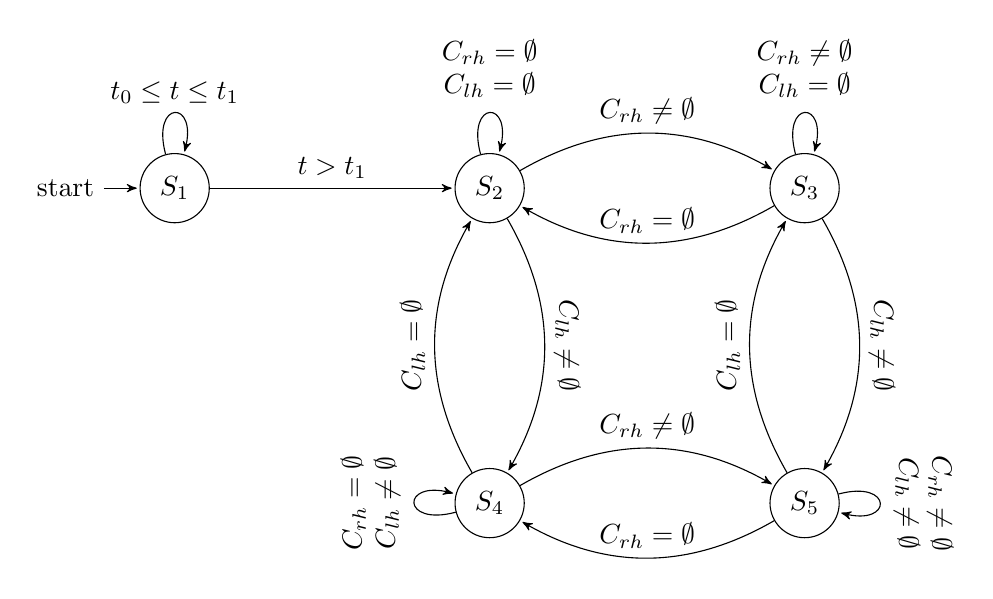
\begin{tikzpicture}[>=stealth',shorten >=1pt,auto,node distance=4cm]
  \node[initial,state] (S1)      {$S_1$};
  \node[state]         (S2) [right of=S1]  {$S_2$};
  \node[state]         (S3) [right of=S2] {$S_3$};
  \node[state]         (S4) [below of=S2] {$S_4$};
  \node[state]         (S5) [below of=S3] {$S_5$};

  \path[->,every node/.style={sloped,anchor=south,auto=false}] 
(S1)  edge [loop above] node {$t_0 \leq t \leq t_1$} (S1)
        edge                     node {$t > t_1$} (S2)
(S2) edge [loop above] node {$\begin{matrix} C_{rh} = \emptyset \\ C_{lh} = \emptyset \end{matrix}$} (S2)
       edge [bend left] node {$C_{rh} \neq \emptyset$} (S3)
       edge [bend left] node {$C_{lh} \neq \emptyset$} (S4)
(S3) edge [loop above] node {$\begin{matrix} C_{rh} \neq \emptyset \\ C_{lh} = \emptyset \end{matrix}$} (S3)
       edge [bend left] node {$C_{lh} \neq \emptyset$} (S5)
       edge [bend left] node {$C_{rh} = \emptyset$} (S2)
(S4) edge [loop left] node {$\begin{matrix} C_{rh} = \emptyset \\ C_{lh} \neq \emptyset \end{matrix}$} (S4)
       edge [bend left] node {$C_{rh} \neq \emptyset$} (S5)
       edge [bend left] node {$C_{lh} = \emptyset$} (S2)
(S5) edge [loop right] node {$\begin{matrix} C_{rh} \neq \emptyset \\ C_{lh} \neq \emptyset \end{matrix}$} (S5)
       edge [bend left] node {$C_{lh} = \emptyset$} (S3)
       edge [bend left] node {$C_{rh} = \emptyset$} (S4);
\end{tikzpicture}
\end{center}

In practice, at start ($t = t_0$) the robot is in state $S_1$ and controls the position and orientation of the pelvis with respect to a world reference frame ($T^{com}_{\bm X}$). Balance is maintained by controlling also the forces and torques exchanged at the right ($T^{rf}_{\bm f}$) and left foot ($T^{lf}_{\bm f}$). A postural tasks ($T^q$) guarantees that the system is not drifting and maintains a posture close to a reference posture. After a predefined amount ($t = t_1$) the system switches to the state $S_2$ by adding two tasks to the set of active tasks: a control of the position and orientation of the right and left hands ($T^{rh}_{\bm X}$ and $T^{lh}_{\bm X}$ respectively). Successive transitions are triggered by the tactile sensors. If no contact are detected on the right and left hand ($C_{rh} = \emptyset$ and $C_{rh} = \emptyset$ respectively) the system remains in $S_2$. A transition from $S_2$ to $S_3$ is performed when the system detects a contact on the right hand ($C_{rh} \neq \emptyset$): in this state the active tasks are the same active in $S_2$ but the right hand position and orientation control ($T^{rh}_{\bm X}$) is replaced with the force control ($T^{rh}_{\bm f}$). Similarly, a transition from $S_2$ to $S_4$ is performed when the system detects a contact on the left hand ($C_{lh} \neq \emptyset$): in this state the active tasks are the same active in $S_2$ but the left hand position and orientation control ($T^{lh}_{\bm X}$) is replaced with the force control ($T^{lh}_{\bm f}$). Finally a transition from either $S_3$ or $S_4$ to $S_5$ is performed whenever the free moving hand perceives a contact so that in this new situation both hands are in contact ($C_{rh} \neq \emptyset$ and $C_{rh} \neq \emptyset$ respectively). In $S_5$ both hands are used to control the interaction forces by activating the tasks $T^{rh}_{\bm f}$ and $T^{fh}_{\bm f}$.

\subsection{Task references} \label{sec:taskReferences}

In this section we discussed how to compute the task references:
$$
{\bm f}^*_{rh}, \quad{\bm f}^*_{lh}, \quad {\bm f}^*_{rf},  \quad {\bm f}^*_{lf}, \quad ^{rh}{\ddot {\bm x}}^*_w, \quad {}^{rh}{\dot {\bm \omega}}_w^* , \quad ^{lh}{\ddot {\bm x}}^*_w, \quad {}^{lh}{\dot {\bm \omega}}_w^*, \quad \ddot {\bm x}^*_{com}.
$$
The proposed definitions assume that for each reference we have an associated desired trajectory which is pre-specified: 
$$
{\bm f}^d_{rh} (t), \quad{\bm f}^d_{lh}(t), \quad {\bm f}^d_{rf}(t),  \quad {\bm f}^d_{lf}(t), \quad ^{rh}{ {\bm x}}^d_w(t), \quad {}^{rh}{ {R}}_w^d(t) , \quad ^{lh}{ {\bm x}}^d_w(t), \quad {}^{lh}{ {R}}_w^d(t), \quad  {\bm x}^d_{com}(t).
$$
The definition of these desired trajectories is discussed in Section \ref{sec:refTrajectories}. In this section we discuss how task references are constructed given the task trajectories.

Let's first discuss how the center of mass reference acceleration $\ddot {\bm x}_{com}^*$ is generated at each instant of time. Given the desired trajectory ${\bm x}_{com}^d (t)$ trajectory we define:
\begin{equation} \label{eq:accRef}
\ddot {\bm x}_{com}^* (t) = \ddot {\bm x}_{com}^d (t) + K_d^{com} \left( \dot {\bm x}_{com}^d (t) - \dot {\bm x}_{com}\right) + K_p^{com} \left( {\bm x}_{com}^d (t) - {\bm x}_{com}\right),
\end{equation}
where $K_p^{com}$ and $K_d^{com}$ are arbitrary positive definite matrices. Similarly, the force reference trajectories ${\bm f}^*_{\cdot} (t)$ are obtained from a desired force trajectory ${\bm f}^d_{\cdot} (t)$:
\begin{equation} \label{eq:fRef}
{\bm f}_{\cdot}^* (t) = {\bm f}_{\cdot}^d (t) + K_i^f \int_0^t \left( {\bm f}_{\cdot}^d (\tau) - {\bm f}_{\cdot} (\tau) \right) d \tau,
\end{equation}
where again $K_i^f$ is an arbitrary positive definite matrix. It is slightly more complicated to define the hands acceleration reference trajectories  ${\ddot {\bm x}}^*_w(t)$, ${\dot {\bm \omega}}_w^* (t)$. The linear acceleration trajectory ${\ddot {\bm x}}^*_w(t)$ can be handled exactly as it was done for the center of mass position exploiting a suitable desired trajectory ${{\bm x}}^d_w(t)$. Angular acceleration trajectories ${\dot {\bm \omega}}_w^* (t)$ are slightly more complicated in considerations of the fact that they are derived from a reference rotation matrix $R^d_w(t) \in SO(3)$. Within this context, we follow the definition in \cite{siciliano2009} and define an orientation error $\bm e_O$ between the desired pose $R^d_w(t) \in SO(3)$ and the current pose $R_w \in SO(3)$ as:
$$
\bm e_O = \sin(\theta) \bm r,
$$
being $\theta$ and $\bm r$ the axis-angle representation of the error rotation $R^d_w(t) R_w^\top$. We have: 
\begin{eqnarray*} 
\dot {\bm e}_O & = & -L \omega + L^\top \omega_d,
\end{eqnarray*}
with:
\begin{eqnarray*} 
L = - \frac{1}{2} \left( S({\bm n_d}) S(\bm n) + S({\bm s}_d) S(\bm s) + S({\bm a}_d) S(\bm a) \right),
\end{eqnarray*}
where $\bm n$, $\bm s$, $\bm a$ (and correspondingly $\bm n_d$, $\bm s_d$, $\bm a_d$) are the columns of $R_w$, i.e. $R_w = \begin{bmatrix} \bm n & \bm s & \bm a \end{bmatrix}$. Similarly, the second derivative of the angular error is given by:
\begin{eqnarray*} 
\ddot {\bm e}_O & = & -\dot L \omega - L \dot \omega + \dot L^\top \omega_d + L^\top \dot \omega_d.
\end{eqnarray*}
where the derivative of $L$ can be expressed as follows (computations omitted):
\begin{multline*} 
\dot L = - \frac{1}{2} \left( S(\omega \times \mathbf n_d) S(\mathbf n) + S({\mathbf n_d}) S(\omega \times \mathbf n) + S(\omega \times \mathbf s_d) S(\mathbf s) + \right. \\ + \left. S({\mathbf s}_d) S(\omega \times \mathbf s) + S(\omega \times \mathbf a_d) S(\mathbf a) + S({\mathbf a}_d) S(\omega \times \mathbf a)\right).
\end{multline*}
The dynamics $\ddot {\bm e}_O + K_d^O \dot {\bm e}_O + K_p^O {\bm e}_O = 0$ can be rewritten as:
\begin{eqnarray*} 
\dot \omega & = & L^{-1} \left( -\dot L \omega  + \dot L^\top \omega_d + L^\top \dot \omega_d + K_d^O \dot {\bm e}_O + K_p^O {\bm e}_O \right),
\end{eqnarray*}
which eventually gives us the following rule for choosing the right and left hand reference trajectories:
\begin{eqnarray*} 
{}^{rh}{\dot {\bm \omega}}_w^* (t) & = & L^{-1} \left( -\dot L {}^{rh}{{\bm \omega}}_w  + \dot L^\top {}^{rh}{{\bm \omega}}_w^d + L^\top {}^{rh}{\dot {\bm \omega}}_w^d + K_d^O \dot {\bm e}_O^{rh} + K_p^O {\bm e}_O^{rh} \right), \\
{}^{lh}{\dot {\bm \omega}}_w^* (t) & = & L^{-1} \left( -\dot L {}^{lh}{{\bm \omega}}_w  + \dot L^\top {}^{lh}{{\bm \omega}}_w^d + L^\top {}^{lh}{\dot {\bm \omega}}_w^d + K_d^O \dot {\bm e}_O^{lh} + K_p^O {\bm e}_O^{lh} \right).
\end{eqnarray*}


\subsection{Task trajectories} \label{sec:refTrajectories}

In this section we discuss how to compute the tasks reference trajectories:
$$
{\bm f}^d_{rh} (t), \quad{\bm f}^d_{lh}(t), \quad {\bm f}^d_{rf}(t),  \quad {\bm f}^d_{lf}(t), \quad ^{rh}{ {\bm x}}^d_w(t), \quad {}^{rh}{ {R}}_w^d(t) , \quad ^{lh}{ {\bm x}}^d_w(t), \quad {}^{lh}{ {R}}_w^d(t), \quad {\bm x}^d_{com}(t).
$$
At this stage of the CoDyCo project, there is no interest in the planning movements but just in controlling them. Therefore, it is out of the scope of the current deliverable to find desired trajectories compatible with the system dynamics, joint limits, motor torque limits and so on. Hands ($T^{rh}_{\bm X}$ or $T^{lh}_{\bm X}$) and center of mass ($T^{rh}_{\bm X}$) trajectories are predefined and assumed to be chosen according to the specific environment chosen for the validation scenario. In particular, the center of mass trajectory ${\bm x}^d_{com}(t)$ is left as a free parameter to be chosen during the validation. Hand trajectories $^{rh}{ {\bm x}}^d_w(t), {}^{rh}{ {R}}_w^d(t), ^{lh}{ {\bm x}}^d_w(t), {}^{lh}{ {R}}_w^d(t)$ are constructed by specifying only the final posture to be reached: $^{rh}{ {\bar{\bm x}}}^d_w, {}^{rh}{ {\bar R}}_w^d, ^{lh}{ \bar{\bm x}}^d_w, {}^{lh}{ \bar {R}}_w^d$. This posture is chosen so as to reach the hand contacts, assumed to be fixed in the world reference frame\footnote{In practice final postures are positions on the positions where the hand contact should occur.}. Whenever either $T^{rh}_{\bm X}$ or $T^{lh}_{\bm X}$ is activated, a new reference trajectory is instantiated corresponding to an interpolation (e.g. a minimum jerk trajectory) from the current hand position to the contact locations; the trajectory duration is left as an open parameter. 

The definition of the interaction force tasks $T^{rf}_{\bm f}$, $T^{lf}_{\bm f}$, $T^{rh}_{\bm f}$, $T^{lh}_{\bm f}$ and the associated reference force values ${{\bm f}}_{rh}^*$, ${{\bm f}}_{lh}^*$, ${{\bm f}}_{rf}^*$, ${{\bm f}}_{lf}^*$ requires more care. The motivation resides in the fact that these tasks are intertwined to the center of mass task $T^{com}_{\bm X}$ through the system dynamics. At each instant of time external forces determine the center of mass acceleration according to the following:
\begin{equation}
m \ddot {\bm x}_{com} = {f}_{rh} + {f}_{lh} + {f}_{rf} + {f}_{lf},
\end{equation}
being $m$ the total mass of the robot and ${f}_{rh}$, ${f}_{lh}$, ${f}_{rf}$ and ${f}_{lf}$ the Cartesian (not the spatial!) forces exchanged by the robot at the contact points. In view of this consideration we need to be careful in choosing reference interaction forces ${{\bm f}}_{rh}^*$, ${{\bm f}}_{lh}^*$, ${{\bm f}}_{rf}^*$, ${{\bm f}}_{lf}^*$ and reference center of mass acceleration $\ddot {\bm x}^*_{com}$. The notation is slightly complicated by the fact that in the different scenario states $S_1$, $\dots$, $S_5$ the meaning of $\bm f$ (and consequently $\bm f^*$) in \eqref{eq:TSID} changes. In particular we have:
\begin{equation}
S_1, S_2: \bm f = \begin{bmatrix} {\bm f}_{rf} \\ {\bm f}_{lf} \end{bmatrix},  \quad
S_3: \bm f = \begin{bmatrix} {\bm f}_{rh} \\ {\bm f}_{rf} \\ {\bm f}_{lf} \end{bmatrix},  \quad
S_4: \bm f = \begin{bmatrix}  {\bm f}_{lh} \\ {\bm f}_{rf} \\ {\bm f}_{lf} \end{bmatrix},  \quad
S_5: \bm f = \begin{bmatrix} {\bm f}_{rh} \\ {\bm f}_{lh} \\ {\bm f}_{rf} \\ {\bm f}_{lf} \end{bmatrix}, 
\end{equation}
where each spatial force has the usual structure $\bm f_i = \left[ \mu_i^\top, f_i^\top \right]^\top$ being $f_i$ the Cartesian force and $\mu_i$ the Cartesian torque always defined in the link reference frame. In the different states, the following constraints on $\bm f^*$ hold with the definitions below:
\begin{itemize}
\item $S_1$ and $S_2$: desired force $\bm f^*$ is such that: 
\begin{equation} C_{S_1} \bm f^* = C_{S_2} \bm f^* = {f}^*_{rf} + {f}^*_{lf} = m \ddot {\bm x}^*_{com}. \label{eq:constraintsS1}\end{equation}
\item $S_3$: desired force $\bm f^*$ is such that:
\begin{equation} C_{S_3} \bm f^* = {f}^*_{rh} + {f}^*_{rf} + {f}^*_{lf} = m \ddot {\bm x}^*_{com}. \label{eq:constraintsS3}\end{equation}
\item $S_4$: desired force $\bm f^*$ is such that: 
\begin{equation} C_{S_4} \bm f^* = {f}^*_{lh} + {f}^*_{rf} + {f}^*_{lf} = m \ddot {\bm x}^*_{com}. \label{eq:constraintsS4}\end{equation}
\item $S_5$: desired force $\bm f^*$ is such that: 
\begin{equation} C_{S_5} \bm f^* = {f}^*_{rh} + {f}^*_{lh} + {f}^*_{rf} + {f}^*_{lf} = m \ddot {\bm x}^*_{com}. \label{eq:constraintsS5}\end{equation}
\end{itemize}
where we defined:
\begin{eqnarray*}
C_{S_1} & = & \begin{bmatrix} 0_{3\times3} & I_{3\times3} & 0_{3\times3} & I_{3\times3} \end{bmatrix}, \\
C_{S_2} & = & \begin{bmatrix} 0_{3\times3} & I_{3\times3} & 0_{3\times3} & I_{3\times3} \end{bmatrix}, \\
C_{S_3} & = & \begin{bmatrix}  C_{S_1} & 0_{3\times3} & I_{3\times3}\end{bmatrix}, \\
C_{S_4} & = & \begin{bmatrix} C_{S_1} & 0_{3\times3} & I_{3\times3}\end{bmatrix}, \\
C_{S_5} & = & \begin{bmatrix} C_{S_3} & 0_{3\times3} & I_{3\times3}\end{bmatrix}. 
\end{eqnarray*}
In general these constraints (deriving from the Newton equation) can be completed with additional constraints which derive from the angular momentum equilibrium, but we left this complete formulation out to simplify the notation. The interested reader should refer to \cite{orin2013}. Similarly to simplify the notation we neglected the effect of gravitational forces, which should be taken into account when balancing forces. Correct computations can be simply obtained by modifying all equations to include a term $m \bm g$ being $\bm g$ the gravitational acceleration. Otherwise all equations still hold referring to the system ``proper acceleration''. 

In the TSID formalism, tasks $T^{rf}_{\bm f}$, $T^{lf}_{\bm f}$, $T^{rh}_{\bm f}$, $T^{lh}_{\bm f}$ can be solved solving \eqref{eq:torquesTSID}-\eqref{eq:dynTSID}-\eqref{eq:contactTSID} at the first stage of the hierarchy (i.e. with maximum priority). However, it is worth observing that the solution of \eqref{eq:torquesTSID}-\eqref{eq:dynTSID}-\eqref{eq:contactTSID} might be in conflict with the center of mass task $T^{com}_{\bm X}$ if it is specified in \eqref{eq:motionTSID} with lower priority with respect to the force task. Therefore, in order to enforce the compatibility of the tasks $T^{rf}_{\bm f}$, $T^{lf}_{\bm f}$, $T^{rh}_{\bm f}$, $T^{lh}_{\bm f}$ and $T^{com}_{\bm X}$, we pre-compute a  reference force $\bm f^*$ compatible with the reference center of mass acceleration $\bm x_{com}^*$. Even if we impose the above constraints on $\bm f^*$, we do not identify a unique solution. Additional constraints or requirements needs to be imposed in order to properly define $\bm f^*$. In order to simplify this ambiguity, the following problem can be solved when at state $S_i$:
\begin{equation} \label{eq:minF}
\bm f^* = \mbox{arg } \min_{\bm f} \| \bm f - \bm f_0 \|^2_W  \mbox{ s.t. } C_{S_i} \bm f= m \ddot {{\bm x}}^*_{com},
\end{equation}
where $\| \cdot \|_W$ denotes a norm weighted with the matrix $W = W^\top >0$. The solution of this optimization is given by:
\begin{equation} 
\bm f^* = m  C_{S_i, W}^\dagger \ddot {{\bm x}}_{com}^*+ (I - C_{S_i, W}^\dagger C_{S_i}) \bm f_0,
\end{equation}
having defined $C_{S_i, W}^\dagger  = \left( C_{S_i}^\top W C_{S_i} \right)^{-1} C_{S_i}^\top W$, the weighted pseudo-inverse of $C_{S_i, W}$. The solution of this optimization gives a set of desired forces $\bm f^*$ which are compatible with the desired center of mass acceleration $\ddot {\bm x}^*_{com} $. 

It was worth noticing that in the above optimization constraints involve only the Cartesian forces while the norm to be minimized is referred to the spatial forces, thus including both Cartesian forces and torques. As a consequence, \eqref{eq:minF} naturally imposes a solution with null Cartesian torques at all contacts. It is worth noting here that all Cartesian forces and torques are defined in a reference frame attached to the rigid link on which the contact is active. Additionally, if these reference frames are properly chosen within the contact support polygon, \eqref{eq:minF} naturally induces the center of pressure condition (sometimes called also the ZMP condition) for all the contacts which guarantees the stability of the contact itself.  

Once a compatible $\bm f^*$ is computed solving \eqref{eq:minF}, tasks $T^{rf}_{\bm f}$, $T^{lf}_{\bm f}$, $T^{rh}_{\bm f}$, $T^{lh}_{\bm f}$ and $T^{com}_{\bm X}$ are simultaneously computed solving the associated optimization \eqref{eq:torquesTSID}-\eqref{eq:dynTSID}-\eqref{eq:contactTSID} which has maximum priority in the hierarchy. Alternatively, a possible solution in a single step consists in solving the following problem:
\begin{subequations} \label{eq:TSID2}
\begin{align} 
\label{eq:torquesTSID2}
\bm {\tau}^* = \mbox{arg } \min_{\bm \tau \in \mathbb{R}^n}\,& \| \bm f \|^2_W \\
\label{eq:dynTSID2}
s.t. \quad M \ddot{\bm q} + h - J_c^T \bm f & = S^T \bm \tau \\
\label{eq:contactTSID2}
  J_c \ddot{\bm q} + \dot{J}_c \dot{\bm q} & = 0 \\
 J_{com} \ddot{\bm q} + \dot{J}_{com} \dot{\bm q} & =  \ddot {\bm x}^*_{com}.
\end{align}
\end{subequations}
The solution of \eqref{eq:TSID2} has strong analogies with the solution of \eqref{eq:minF} and \eqref{eq:torquesTSID}-\eqref{eq:dynTSID}-\eqref{eq:contactTSID} but a complete analysis of the underlying similarities is out of the scope of the present report. 

In order to avoid discontinuities in the desired forces to be tracked by the controller we should chose the trajectories ${{\bm f}}_{rh}^*(t)$, ${{\bm f}}_{lh}^*(t)$, ${{\bm f}}_{rf}^*(t)$, ${{\bm f}}_{lf}^*(t)$ so that at the moment of task switching the desired force equal the current one. In order to do so, we simply exploit the fact that at any time, measurements $\bm f$, $ \ddot {\bm x}_{com}$ should satisfy the equilibrium condition $C_{S_i} \bm f = m \ddot {\bm x}_{com}$. Therefore, at the switching instant $t_s$ we can simply solve \eqref{eq:minF} with $\bm f_0 = C_{S_i} \bm f (t_s) $ and $\ddot {\bm x}^*_{com} = \ddot {\bm x}_{com}(t_s)$ to obtain a solution $\bm f^* = \bm f (t_s)$. The values of $\ddot {\bm x}^*_{com}$ and $\bm f_0$ are then obtained as described in Section \ref{sec:taskReferences} as the output of a $PID$ filter on the difference between desired trajectories $\ddot {\bm x}^d_{com} (t)$, $\bm f^d(t)$ and current values $\ddot {\bm x}_{com}$, $\bm f$. In particular, according the definitions that we gave in \eqref{eq:accRef} and \eqref{eq:fRef} the final reference for forces and accelerations will be:
\begin{eqnarray*} 
\ddot {\bm x}_{com}^* (t) &=& \ddot {\bm x}_{com}^d (t) + K_d^{com} \left( \dot {\bm x}_{com}^d (t) - \dot {\bm x}_{com}\right) + K_p^{com} \left( {\bm x}_{com}^d (t) - {\bm x}_{com}\right), \\
{\bm f}_0 (t) & = & {\bm f}^d (t) + K_i^f \int_{t_s}^t \left( {\bm f}^d (\tau) - {\bm f} (\tau) \right) d \tau,\\
\bm f^* & =&  m  C_{S_i, W}^\dagger \ddot {{\bm x}}_{com}^*+ (I - C_{S_i, W}^\dagger C_{S_i}) \bm f_0.
\end{eqnarray*}
At the switching instant $t_s$ we choose $\bm f^d = \bm f $, $\ddot {\bm x}^d_{com} = \ddot {\bm x}_{com}$, $\dot {\bm x}^d_{com} = \dot {\bm x}_{com}$, $ {\bm x}^d_{com} = {\bm x}_{com}$ so as to obtain $\bm f^* = \bm f$ (remeber that $\bm f$, $ \ddot {\bm x}_{com}$ are always compatible). Then we can choose $\bm f^d (t)$ and $\ddot {\bm x}^d_{com}(t)$ arbitrarily with the guarantee that the resulting $\bm f^*$ and $\ddot {\bm x}_{com}^*$ will always be dynamically consistent.

\subsection{Task prioritization} \label{sec:taskPrioritization}

In the TSID framework, control tasks are executed with a lexicographic priority, i.e. tasks with higher priority should be satisfied at the expenses of the tasks with lower priority. In order to represent $T_i$ with a lower lexicographic priority with respect to $T_j$ we use the notation $T_i \prec T_j$. In consideration of what discussed above, tasks force tasks $T^{rf}_{\bm f}$, $T^{lf}_{\bm f}$, $T^{rh}_{\bm f}$, $T^{lh}_{\bm f}$ and center of mass tasks $T^{com}_{\bm X}$ are grouped in a unique optimization which we denote $T^{com}_{\bm f}$. In the different states, priorities are handled as follows:

\begin{itemize}
\item $S_1$ and $S_2$: $T^q \prec T^{com}_{\bm f}$.
\item $S_2$: $T^q \prec T^{lh}_{\bm X}  \prec  T^{rh}_{\bm X} \prec T^{com}_{\bm f} $.
\item $S_3$: $T^q \prec T^{lh}_{\bm X}  \prec T^{com}_{\bm f} $.
\item $S_4$: $T^q \prec T^{rh}_{\bm X}  \prec T^{com}_{\bm f} $.
\item $S_5$: $T^q \prec T^{com}_{\bm f} $.
\end{itemize}

\subsection{Alternative controller formulation}
The Task Space Inverse Dynamics (TSID) can be formulated in a fashion where the ordering of the tasks priorities can be based on soft priorities rather than on a strict lexicographic order. The control problem can still be written as an optimization problem under constraints and its resolution only requires one optimization level, independently from the number of tasks to be achieved. The work of Joseph Salini \cite{salini2012} at UPMC lays the foundation of this alternative formulation paradigm. Figure~\ref{fig:joseph} illustrates the principles of this formulation where a weight is associated to each task accordingly to its importance and can be modulated using a rule-based high level decision making process.\\

\begin{figure*}
\begin{center}
\centering
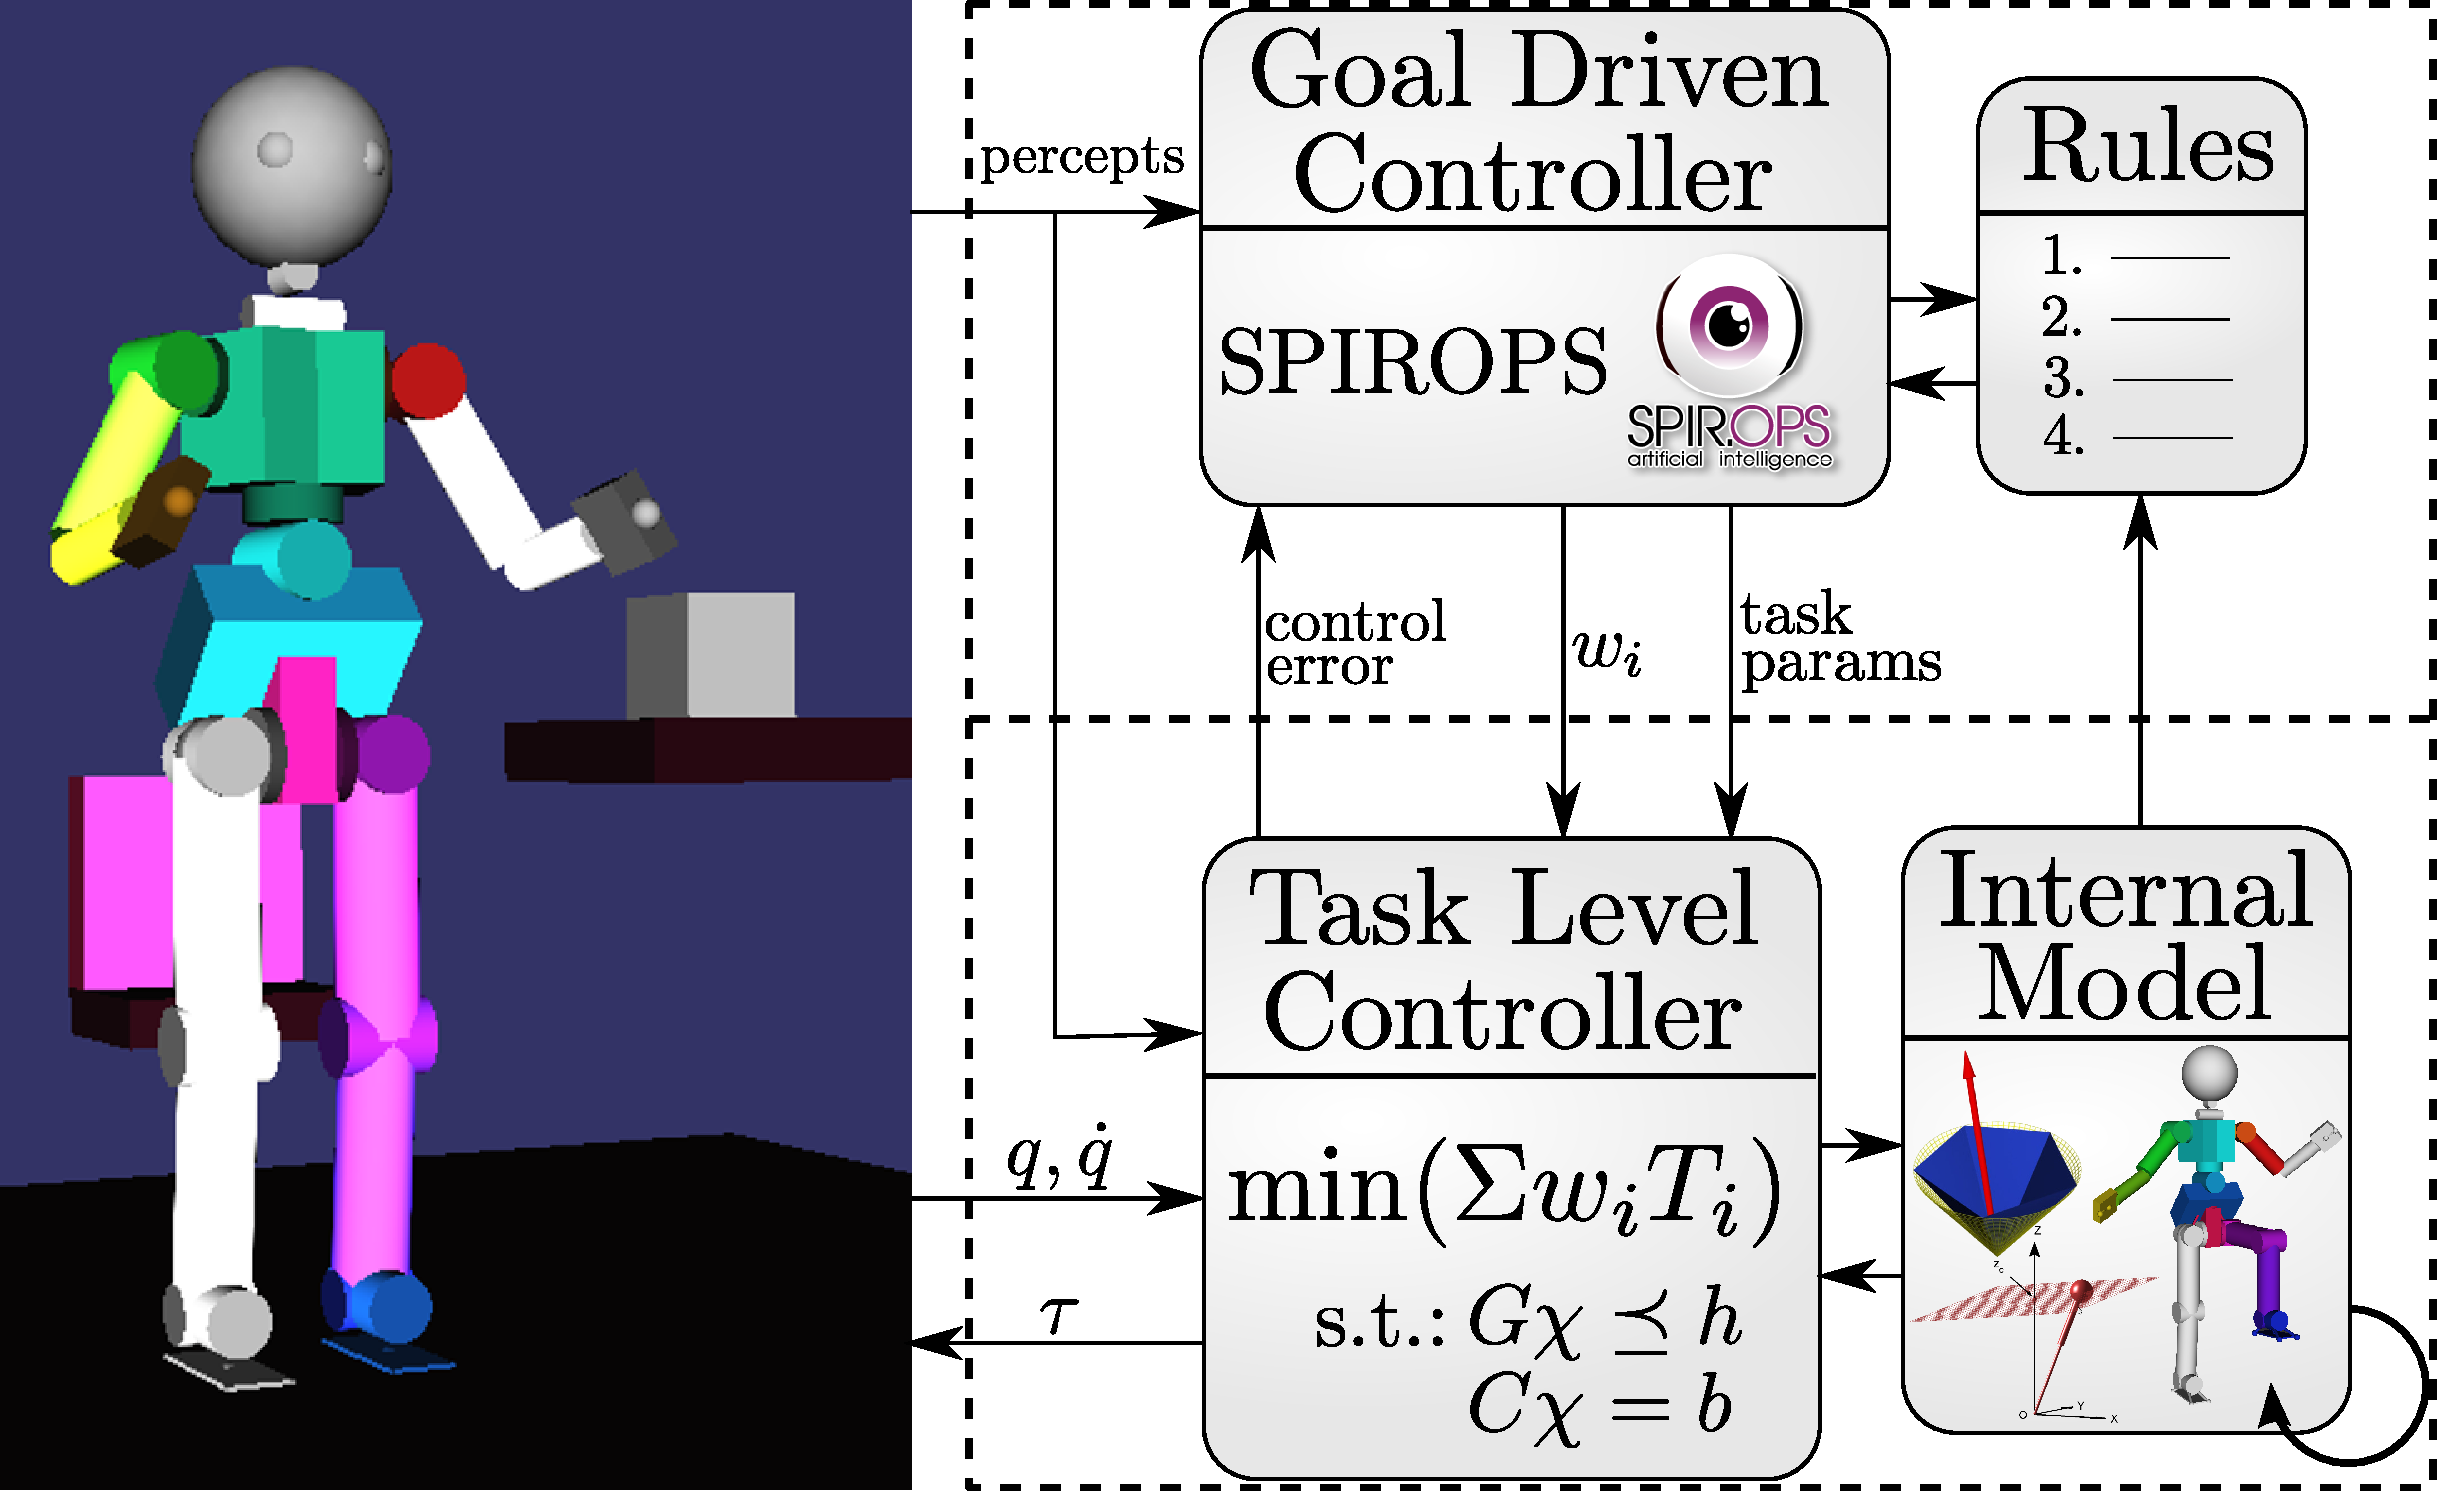
\includegraphics[width=0.8\textwidth]{images/global_architecture.pdf} 
\caption{Global architecture of the soft hierarchy Task Space Inverse Dynamics control scheme developed at UPMC.}
\label{fig:joseph}
\end{center}
\end{figure*}

While appealing, the work of J. Salini can not guarantee strict priorities between tasks. On the other hand, control approaches based on strict hierarchies induce discontinuities in the control input when modifying the ordering of the hierarchy and require to solve as many optimization problems as the number of tasks. In order to solve these issues and as a contribution to WP3, UPMC recently developed a controller named Generalized Smooth Hierarchical Control (GSHC) bridging the gap between strict and soft hierarchy Task Space Inverse Dynamics controllers. The GHSC algorithm, submitted to the IEEE Transaction on Robotics journal \cite{liu2013}, provides with a control framework such that:
\begin{itemize}
	\item it can handle multiple tasks with strict and soft priorities;
	\item smooth and simultaneous rearrangements of multiple task priorities can be achieved easily (by the smooth variations of relevant bounded scalar values);
	\item smooth insertion and deletion of tasks can be performed;
	\item various constraints imposed by the robot body (joint limits, actuation capabilities...) and the environment (contacts to maintain, obstacles to avoid...) can be respected.
\end{itemize}

The first year demo described in this delievrable thus also benefits from this alternative controller. It is being intensively tested on a simulated iCub in the XDE simulator at UPMC before being transfered to IIT for an implementation on the real robot. The validation scenario is also being investigated (see Figure~\ref{fig:xde}) . For example, UPMC is testing how to smoothly sequence force and position tasks when contact is detected. UPMC also has developed a set of tools to rapidly prototype and test different behaviors of the robot by acting on tasks priority parameters (see Figure~\ref{fig:params}).

\begin{figure*}[h]
\begin{center}
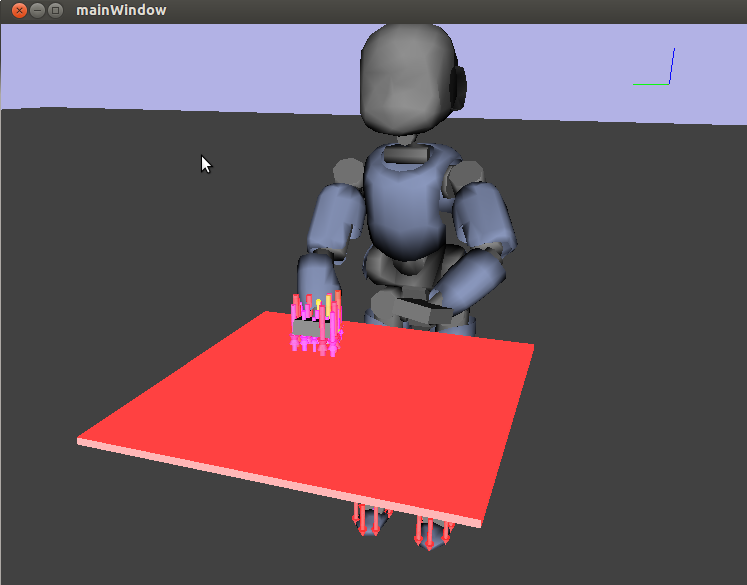
\includegraphics[width=0.3\hsize]{images/s5.png}
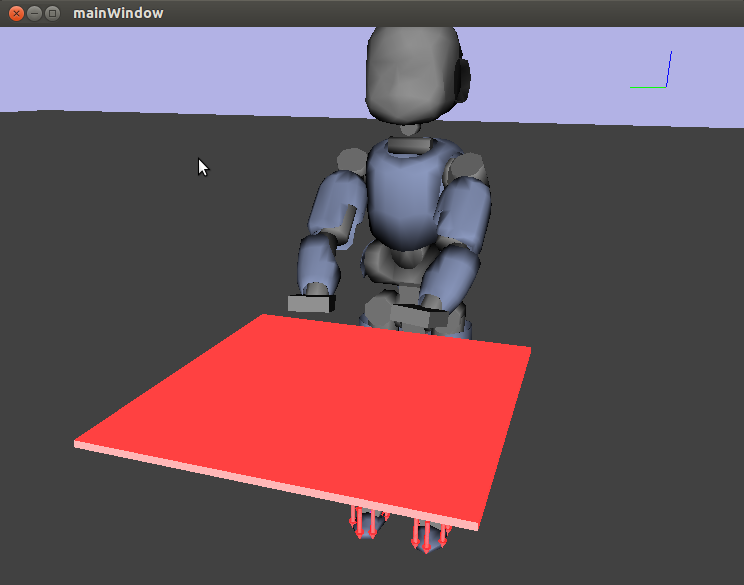
\includegraphics[width=0.3\hsize]{images/s6.png}
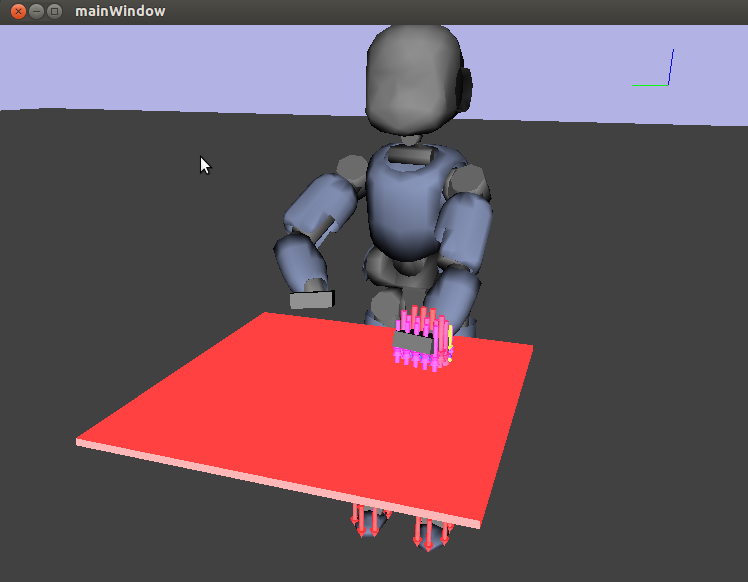
\includegraphics[width=0.3\hsize]{images/s4.png}

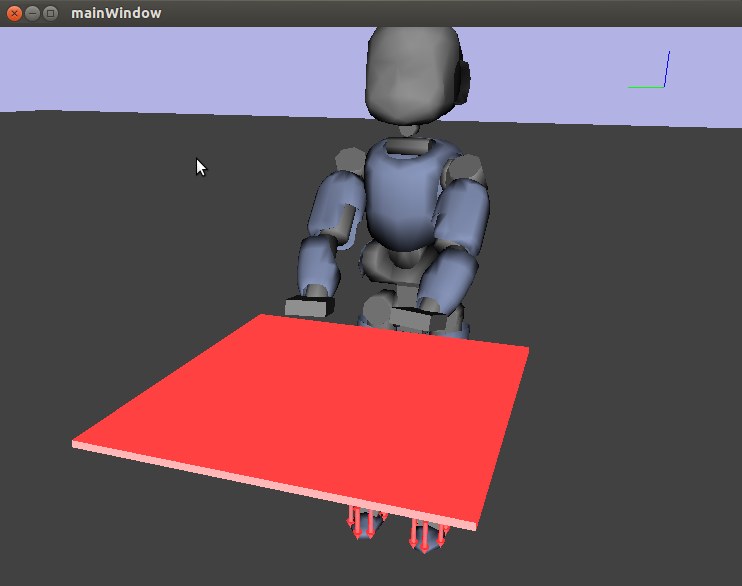
\includegraphics[width=0.3\hsize]{images/s3.png}
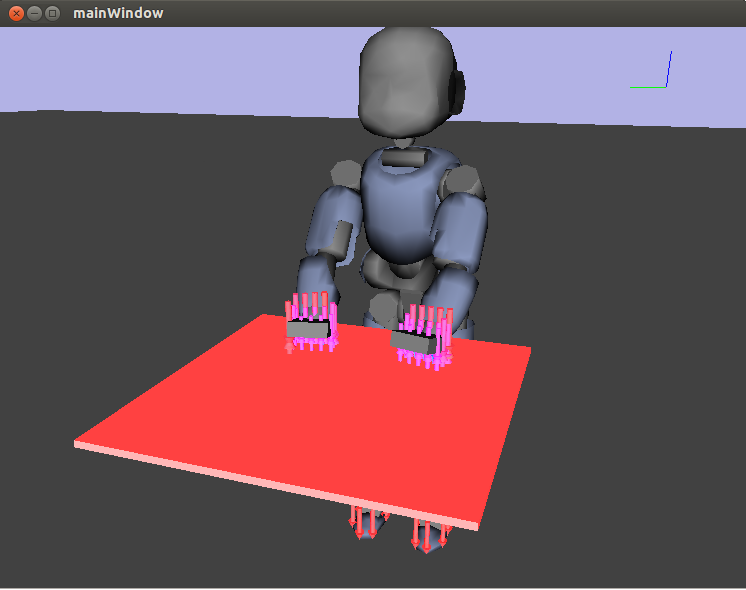
\includegraphics[width=0.3\hsize]{images/s2.png}
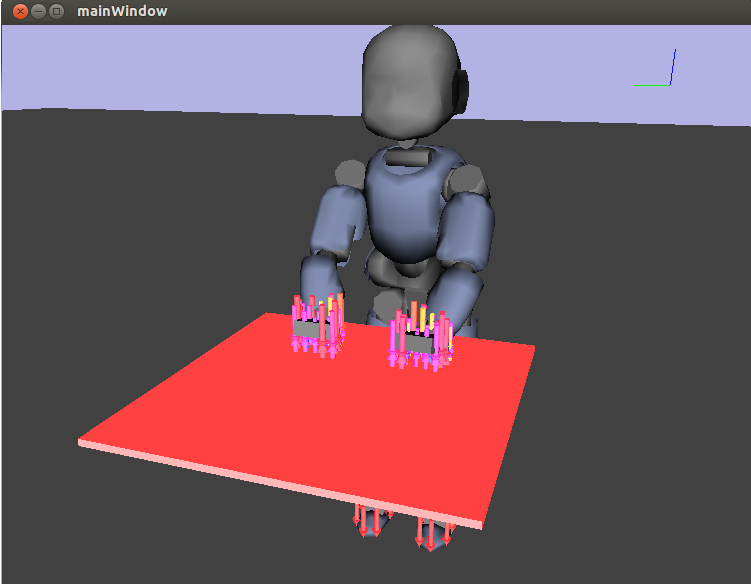
\includegraphics[width=0.3\hsize]{images/s1.png}
\end{center}
\caption{Screenshots of the validation scenario simulated in XDE.}
\label{fig:xde}
\end{figure*}

\begin{figure*}
\begin{center}
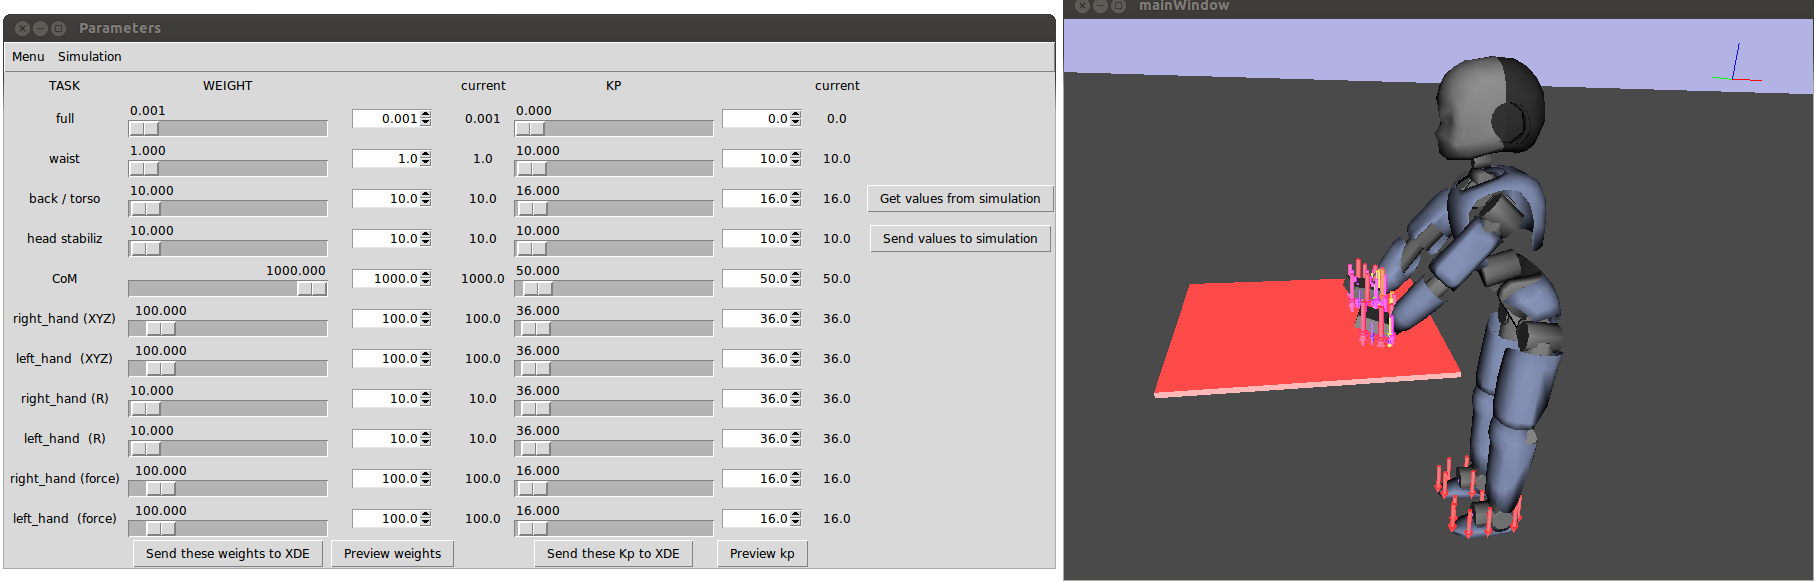
\includegraphics[width=0.9\hsize]{images/s12.png}
\end{center}
\caption{Tuning of the task priority parameters in XDE.}
\label{fig:params}
\end{figure*}

\bibliographystyle{apalike}
\bibliography{D5.1}

\newpage \appendix

\section{Center of pressure: $\bm {CoP}$}

In this Appendix we recall some concepts that have been extensively discussed in the CoDyCo deliverable D2.1, where the main focus is on human motion analysis. Remarkably, concepts like center of pressure and (fictitious) zero moment point apply to both humans and robots thus representing a strong modeling analogy between the two fields of research. In general, all dynamic principles (Newton-Euler equation, energy, work, forces, torques, etc.) represent a abstraction layer that allows the CoDyCo consortium to have a common set of tools which can be independently applied to both humans and robots. 

\subsection{$\bm{CoP}$ definition}

In order to define the center of pressure it is first necessary to define the pressure. Pressure is a scalar quantity, defined as the amount of force acting perpendicularly per unit area. Let's assume that a set of distributed forces acts on a surface $\mathcal S$ and let $\bm s$ be a point on the surface, i.e. $\mathbf s \in \mathcal S$. Let's denote with $f_n(\mathbf s)$ the component of $f(\mathbf s)$ orthogonal to $\mathcal S$ in $\mathbf s$. Given $\mathbf s \in \mathcal S$, assuming an element $\Delta S(\mathbf s)$ of infinitesimal area centered in $\mathbf s$, let $f_n(\Delta S,\mathbf s)$ be the orthogonal force acting on $\Delta S(\mathbf s)$. The pressure $p$ in $\mathbf s$ is defined as:
$$
p(\mathbf s) = \lim_{\Delta S \rightarrow 0} \frac{f_n(\Delta S, \mathbf s)}{\Delta S} \qquad \mathbf s \in \Delta S.
$$
Under this definition, the center of pressure $CoP$ with respect to the the reference frame $\Sigma_1$ is defined as:
$$
CoP_1 = \frac{\int_{\mathcal S} \mathbf s_1 \cdot p(\mathbf s) dS}{\int_{\mathcal S} p(\mathbf s) dS},
$$
where $\mathbf s_1$ indicates the position of $\mathbf s$ in $\Sigma_1$. If $\mathcal S$ is a three dimensional surface, the $CoP$ is a three dimensional point. It is totally equivalent to the concept of the center of mass, but instead of being related to the first order moment of the mass it involves the first order moment of the pressure. A number of interesting properties follow and in particular if $\mathcal S$ is convex then $CoP \in \mathcal S$. Another important property is $CoP_2 ={}^2 T_1 \cdot CoP_1$ if $^2 T_1$ transforms from $\Sigma_1$ to $\Sigma_2$. The total orthogonal force $f_n$ acting on the surface is given by:
$$
f_n = \int_{\mathcal S} p(\mathbf s) dS,
$$
and the global force $\mathbf f$ is the sum of the global normal force ($\mathbf f_n$) and the global tangential force ($\mathbf f_t$) due to the tangential elementary forces $\mathbf t(s)$:
$$
\mathbf f = \mathbf f_n +\mathbf f_t = f_n \cdot \mathbf n + \int_{\mathcal S} \mathbf t(\mathbf s) dS = \int_{\mathcal S} p(\mathbf s) \cdot \mathbf n + \mathbf t(\mathbf s) dS,
$$
being $\mathbf n$ the surface normal. Clearly we have $\langle \mathbf t(\mathbf s), \mathbf n \rangle=0$, for all $\mathbf s \in \mathcal S$. Also the global moment $\boldsymbol\mu$ can be decomposed in two different contributions, one due to orthogonal forces $\boldsymbol\mu_n$ and one due to tangential force $\boldsymbol\mu_t$. On $\Sigma_1$ we have:
$$ 
\boldsymbol\mu_{n,1} = \left( \int_{\mathcal S} p(\mathbf s) \mathbf s_1 dS \right) \times \mathbf n = CoP_1 \times \left( f_n \cdot \mathbf n \right), \qquad \boldsymbol\mu_{t,1} = \int_{\mathcal S}  \mathbf s_1 \times \mathbf t(\mathbf s) dS. 
$$
In the case of flat surfaces $\mathcal S$, it can be shown \cite{sardain2004} that the $CoP$ is the unique point $C \in \mathcal S$ on which $\boldsymbol\mu_{n,C} = 0$\footnote{We can prove that indeed $\boldsymbol\mu_{n,CoP} = 0$. First of all, let's observe that:
$$ 
\boldsymbol\mu_{n,2} = \boldsymbol\mu_{n,1} + f_n \cdot \mathbf n \times \mathbf {}^2 \mathbf s_{1},
$$
where ${}^2 \mathbf s_{1}$ is the vector from $\Sigma_1$ to $\Sigma_2$. We have:
$$
\boldsymbol\mu_{n,CoP} = \left( \int_{\mathcal S} p(\mathbf s) \mathbf s_1 dS \right) \times \mathbf n  + \int_{\mathcal S} p(\mathbf s) \cdot \mathbf n dS \times \frac{\int_{\mathcal S} \mathbf s_1 \cdot p(\mathbf s) dS}{\int_{\mathcal S} p(\mathbf s) dS} = 0.
$$}. Equivalently, we can say that the $CoP$ is the unique point $C \in \mathcal S$ on which  $\boldsymbol\mu_{C} = \boldsymbol\mu_{t,C}$, i.e. the total torque $\boldsymbol\mu_{C}$ is orthogonal to $\mathcal S$. It is here worth noticing that on flat surfaces the torque due to normal forces $\boldsymbol\mu_{t}$ is parallel to the plane normal $\mathbf n$ while the torque due to tangential forces $\boldsymbol\mu_{n}$ lies on the plane. 

\subsection{$\bm {CoP}$ and dynamic equilibrium}

The concept of center of pressure is often related to the concept of dynamic equilibrium for a free floating articulated body. Within the multiple point of views proposed in literature we primarily follow the one in \cite{sardain2004}. Therefore, we do not make any formal distinction between the concept of $CoP$ (center of pressure) and the concept of $ZMP$ (zero moment point) because, as it is clearly stated in \cite{sardain2004}, ``$CoP$ and the $ZMP$ are the same point. [$\dots$] This fact does not admit any discussion, it is true whatever the stability of the balance is, and in particular it is true when the walker is falling down, as long as a contact exists with the ground''. What might generate confusion is that Vukobratovi\'c, the author that introduced the concept of $ZMP$, also introduced the concept of fictitious $ZMP$ lately renamed computed zero moment point ($cZMP$, see chapter sixteen of the handbook of robotics \cite{handbook2008}). 

Similarly to the $CoP$ the $cZMP$ is a point associated with a force/torque couple $\boldsymbol f^b, \boldsymbol\mu^b$ represented in a given reference frame $\Sigma_b$. Similarly to the $CoP$ its definition passes through an associated plane $\mathcal S$ (the planar support). In particular the $cZMP$ is defined as the unique point $C \in \mathcal S$ where $\boldsymbol\mu^b_C$ is orthogonal to $\mathcal S$. The difference between the $CoP$ and the $cZMP$ relies on the fact that the $CoP$ is defined on the force/torque ($\boldsymbol f, \boldsymbol\mu$) that the foot exchanges with the ground, while the $cZMP$ is defined on all the other forces/torques ($\boldsymbol f^b, \boldsymbol\mu^b$) that the foot exchanges with the articulated body. At the foot center of mass the usual Newton-Euler equations should hold:
$$
m_f \bm a_f = \boldsymbol f^b + \boldsymbol f, \qquad \bm I_f \dot {\boldsymbol \omega}_f =  \boldsymbol \mu^b + \boldsymbol \mu,
$$
where all quantities are referred to a reference frame in the foot center of mass, $m_f$ is the total mass of the foot, $\bm a_f$ is the foot linear acceleration, $\bm I_f $ is the foot inertia tensor and $\dot {\boldsymbol \omega}_f $ the foot angular acceleration. 

If the foot is at equilibrium ($\dot {\boldsymbol \omega}_f = \bm a_f = 0$) then the $CoP$ and the $cZMP$ are defined on equal and opposite force/torque couples since we have ($\boldsymbol f^b, \boldsymbol\mu^b$) = ($-\boldsymbol f, -\boldsymbol\mu$). It can be shown\footnote{Given a force/torque couple $\boldsymbol f, \boldsymbol\mu$ and a plane $\mathcal S$ the associated $CoP$ is the same associated with the opposite force/torque couple $-\boldsymbol f, -\boldsymbol\mu$ on the same plane $\mathcal S$.} that in this case the $CoP$ and the $cZMP$ coincide. As a consequence the $cZMP$ lies in the foot support polygon. 

Vice-versa, let's prove that if $cZMP$ is outside the support polygon then necessarily either $\dot {\boldsymbol \omega}_f \neq 0$ or $\bm a_f \neq 0$ and therefore the foot is not in equilibrium. Suppose by contradiction that $\dot {\boldsymbol \omega}_f = \bm a_f = 0$. As previously pointed out $CoP$ and $cZMP$ coincide and since the $CoP$ is necessarily within the support polygon we conclude that the $cZMP$ is also within the support polygon thus leading to the contradiction. 

Finally, we would like to give sufficient conditions for the foot stability. In particular, can we conclude that if the $cZMP$ is within the support polygon then the foot is at equilibrium? Unfortunately this conclusion cannot be drawn stated as it is. The main motivation resides in the fact that the $cZMP$ might be associated with a force/torque couple $\boldsymbol f^b, \boldsymbol\mu^b$ whose tangential force components ($\boldsymbol f_t$) are outside the friction cones. Remarkably, this might always be the case since the zero moment point condition does not involve the tangential forces. Similarly,  the $cZMP$ might be associated with a force/torque couple $\boldsymbol f^b, \boldsymbol\mu^b$ whose normal torque component ($\boldsymbol \mu_t$) is outside the friction cones. Again, this might always be the case since the zero moment point condition does not involve the torque component normal to the contact plane. What it can be proven (but the complete proof is outside the scope of the current deliverable) is that if the $cZMP$ is inside the support polygon and if the the associated force/torque couple $\boldsymbol f^b, \boldsymbol\mu^b$ have tangential force components ($\boldsymbol f^b_t$) and normal torque components ($\boldsymbol \mu^b_t$) compatible with the friction cone, then the foot is at equilibrium.

\end{document}

%%% Local Variables:
%%% mode: latex
%%% TeX-master: t
%%% save-place: t
%%% End:
